% SOURCE_AUTHORITY: sga5_fr_workpass.tex, lines 1254--1371 (LF-normalized unit).
Vejamos agora que o emparelhamento (4.7.1) é \textquotedblleft perfeito\textquotedblright{}, isto é, que a seta (4.7.1)' identifica $\R\Gamma(V,i_!G')[-1]$ com $\underline{D}_x\R\Gamma(U,G)$. Suponhamos, de fato, como podemos fazê-lo, que
\[
G=(ji)^*F,
\]
com $F\in\ob\D_c^b(X)$. Colocando $F'=\underline{D}_X(F)$ e $F'_{U,X}=(ji)_!G'$, temos a sequência exata
\[
(4.7.9)\qquad 0\longrightarrow F'_{U,X}\longrightarrow F'\longrightarrow F'|Y\longrightarrow0,
\]
que dá origem a um triângulo distinguido
\[
(b)\qquad
\begin{tikzcd}
& \R\Gamma_x(F'_{U,X}) \arrow[dr] \\
\R\Gamma_x(F'|Y) \arrow[ur,"{+1}"] && \R\Gamma_x(F') \arrow[ll]
\end{tikzcd}
\]
Por definição de $\R\Gamma_x$, temos
\[
\R\Gamma_x(F'_{U,X})=\R\Hom(A_x,F'_{U,X});
\]
Portanto, usando (4.7.7) e o fato de que $(F'_{U,X})_x=\R\Gamma(X,F'_{U,X})=0$, obtém-se um isomorfismo canônico
\[
\R\Hom(A_{V,X},F'_{U,X})[1]\xrightarrow{\sim}\R\Gamma_x(F'_{U,X}).
\]
Mas tem-se
\[
\begin{aligned}
\R\Hom(A_{V,X},F'_{U,X})&=\R\Hom(j_!A_V,j_!i_!G')\\
&\simeq\R\Hom(A_V,i_!G')\qquad\text{por dualidade (SGAA~XVIII~3.1.10)},
\end{aligned}
\]
de onde finalmente se obtém um isomorfismo canônico
\[
(4.7.10)\qquad \R\Gamma_V(i_!G')[-1]\xrightarrow{\sim}\R\Gamma_x(F'_{U,X}).
\]
Por outro lado, tem-se a sequência exata
\[
(4.7.11)\qquad 0\longrightarrow A_{U,X}\longrightarrow A_X\longrightarrow A_Y\longrightarrow0,
\]
que dá origem a um triângulo distinguido
\[
(a)\qquad
\begin{tikzcd}
& \R\Gamma(U,F|U) \arrow[dl,"{+1}"'] \\
\R\Gamma_Y(F) \arrow[rr] && \R\Gamma_X(F) \arrow[ul]
\end{tikzcd}
\]
Em virtude de (4.7.1) e (4.7.10), tem-se um emparelhamento natural
\[
(4.7.12)\qquad \R\Gamma(U,F|U)\times\R\Gamma_x(F'_{U,X})\longrightarrow A.
\]
Em virtude de (4.6.1), tem-se um emparelhamento perfeito
\[
(4.7.13)\qquad \R\Gamma_Y(F)\times\R\Gamma_x(F'|Y)\longrightarrow A.
\]
Por último, pela fórmula de indução ordinária (1.12 b) (i)), tem-se um emparelhamento perfeito
\[
(4.7.14)\qquad \R\Gamma(X,F)\times\R\Gamma_x(F')\longrightarrow A.
\]
O leitor que tenha a paciência de orientar-se neste dédalo de \textquotedblleft setas canônicas\textquotedblright{} verificará que os emparelhamentos (4.7.12), (4.7.13) e (4.7.14) são \textquotedblleft compatíveis\textquotedblright{} com as setas dos triângulos (a) e (b), e, por conseguinte, que os emparelhamentos (4.7.12) e (4.7.1) são perfeitos.

O emparelhamento dos triângulos (a) e (b) dá origem a duas sequências exatas \textquotedblleft transpostas uma da outra\textquotedblright{}:
\[
(4.7.15)\qquad \cdots\longrightarrow \H_Y^i(X,F)\longrightarrow\H^i(X,F)\longrightarrow\H^i(U,F)\longrightarrow\cdots
\]
\[
\cdots\longleftarrow \H_x^{-i}(Y,F'|Y)\longleftarrow\H_x^{-i}(X,F')\longleftarrow\H^{-i-1}(V,F'_{U,V})\longleftarrow\cdots.
\]
Em resumo, podemos enunciar:

\begin{statement}{Proposição 4.7.16}
Seja $X$ um esquema estritamente local noetheriano, de ponto fechado $x$. Sejam $Y$ um fechado não vazio de $X$, $U=X-Y$, $V=X-x$, e $i:U\to V$ e $j:V\to X$ as inclusões canônicas. Seja $K_X$ um complexo dualizante sobre $X$ normalizado em $x$ (de onde se obtêm complexos dualizantes associados sobre $V,U,Y$). Para $G\in\ob\D_c^b(U)$, tem-se um emparelhamento perfeito:
\[
(*)\qquad \R\Gamma(U,G)\times\R\Gamma(V,i_!G')[-1]\longrightarrow A
\]
(onde $G'=\underline{D}_U(G)$). Se $G=F|U$, onde $F\in\ob\D_c^b(X)$, temos um isomorfismo canônico
\[
(**)\qquad \R\Gamma(V,i_!G')[-1]\xrightarrow{\sim}\R\Gamma_x(F'_{U,X})
\]
(onde $F'=\underline{D}_X(F)$ e $F'_{U,X}=(ji)_!(F'|U)=(ji)_!(G')$), e um emparelhamento perfeito entre os triângulos distinguidos
\begin{center}
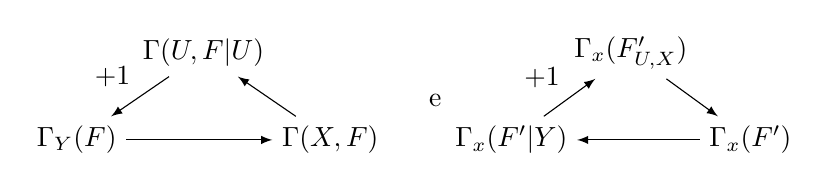
\begin{tikzpicture}[>=latex,scale=0.92,baseline=(current bounding box.center)]
\node (aT) at (0,1.2) {$\R\Gamma(U,F|U)$};
\node (aL) at (-1.75,0) {$\R\Gamma_Y(F)$};
\node (aR) at (1.75,0) {$\R\Gamma(X,F)$};
\draw[->] (aL) -- (aR);
\draw[->] (aR) -- (aT);
\draw[->] (aT) -- node[above left] {$+1$} (aL);
\node at (3.2,0.55) {e};
\node (bT) at (5.9,1.2) {$\R\Gamma_x(F'_{U,X})$};
\node (bL) at (4.25,0) {$\R\Gamma_x(F'|Y)$};
\node (bR) at (7.55,0) {$\R\Gamma_x(F')$};
\draw[->] (bT) -- (bR);
\draw[->] (bR) -- (bL);
\draw[->] (bL) -- node[above left] {$+1$} (bT);
\end{tikzpicture}
\end{center}
compatível com o emparelhamento $(*)$ e o isomorfismo $(**)$, e que dá lugar a duas sequências exatas transpostas uma da outra (4.7.15).
\end{statement}

\begin{statement}{Observação 4.7.17}
No caso particular em que $Y=\{x\}$, o emparelhamento (4.7.1) define-se sob a única hipótese de que $K_X$ esteja normalizado em $x$ (e não seja necessariamente dualizante), isto é, que $\R\Gamma_x(K_X)\simeq A$ (sendo dado o isomorfismo): de fato, o isomorfismo (4.7.2) (que utilizava a bidualidade) reduz-se à identidade. Como o emparelhamento (4.7.14) é perfeito em qualquer caso, vê-se, pois, que a dualidade local sobre $X$ (na forma (4.2.2)') equivale à dualidade \textquotedblleft global\textquotedblright{} sobre $U=X-x$, isto é, ao fato de que o emparelhamento (4.7.1)
\[
\R\Gamma(U,G)\times\R\Gamma(U,G')[-1]\longrightarrow A
\]
seja perfeito ou, equivalentemente, que os emparelhamentos
\[
\H^i(U,G)\times\H^{-i-1}(U,G')\longrightarrow A
\]
sejam perfeitos.

Suponhamos que se dispõe sobre $X$ de um complexo dualizante $K_X$ normalizado em $x$. Se $X$ é excelente e $U$ regular de dimensão $d$ (de modo que $x$ pode ser uma singularidade isolada), deve ser possível verificar que $K_U=K_X|U$ é canonicamente isomorfo a $(\mu_n)_U^{\otimes d}[2d]$ (verifica-se facilmente, em qualquer caso, se $X$ é a localização estrita de um esquema localmente de tipo finito sobre um corpo de car.~0). Então a dualidade local sobre $X$ implica que, para todo $A_U$-módulo localmente constante construtível $G$, têm-se emparelhamentos perfeitos:
\[
\H^i(U,G)\times\H^{2d-1-i}(U,G^\circ)\longrightarrow A,
\]
(onde $G^\circ=\uHom(G,(\mu_n)_U^{\otimes d})$), que correspondem formalmente à dualidade de Poincaré sobre um esquema de dimensão $2d-1$.
\end{statement}
